\section{Stereo vision}

The structure of an object can be extracted relatively easily from distinct features that can be detected with several cameras [CITE].

Three-dimensional capture means in general the way of recording a sequence of movements of a real-life target or scene.


This chapter introduces the methods for seeing three-dimensional structures from stereo setups, consisting of two or more cameras.
The configuration of a proper setup with two is described and it is extended to the multi-view domain.
The previous chapter described how to record a view of a scene with a camera. From now on, the term camera refers to a particular camera configuration, which can be a single physical camera moved to different locations.

\subsection{Coordinate systems and transforms}

The camera is a projective object located somewhere in the imaged scene.
\textit{intrinsic parameters} model the properties of projection, but it does not take into account the camera location in any global coordinate system.
The \textit{extrinsics parameters} contain the camera location and rotation in another global coordinate system, modeled as a matrix.
This is especially advantageous when there are more than one cameras and their coordinates must be related.
\cite{hartley03multiview,heyden2005multiple}
This chapter brings asdfgja basic transforms whose results are needed in the later reconstruction steps.

Calibration is often specified with a camera projection matrix, or several separate matrices.
It may be convenient to store intrinsics and extrinsics separately if the intrinsic matrix is constant for several pictures, for example.


\simplefig{h}{%
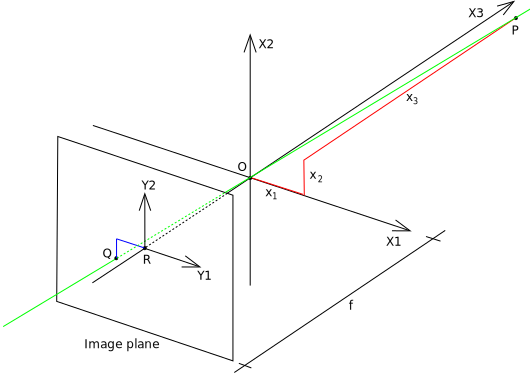
\includegraphics[width=0.7\textwidth]{gfx/pinhole3d}
}{fig:pinhole3d}
{Pinhole camera geometry. Camera coordinate system origin at O, axis X3 points towards the optical axis, Y1 and Y2 point to image plane axes and R is the principal point, at the image center. The point P projects to Q, as well as everything else on the line joining them. The image plane is f units away from camera origin; f is called the focal length.}

What the camera does.

Homogenous point description here, [dubrofsky] homography estimation is nice, also refer hartley/zisserman

In computer graphics and vision, points and directions are usually described in homogenous coordinates. Translation, perspective projection, rotation, and other operations are conveniently described by using an additional dimension, of which usually the last element is 1: $(x, y, z, 1)$. All points $(xw, yw, zw, w)$ map to the same point $(x, y, z)$ something something.

Homography definition (mapping of points and lines in $P^2$)

The imaging process essentially captures a projection to a flat two-dimensional plane of the camera's view, as described in section \ref{sec:imaging}.
When relating points between different cameras that view the same scene, their relational positions and rotations must be known.
One of the cameras is often conveniently chosen as the origin of a global coordinate frame, so that its extrinsic parameters become unity transforms (e.g. opencv stereo).
Each three-dimensional point in the world is transformed to the small sensor or film inside the camera, which is then digitized to a discrete two-dimensional grid of pixels. The size of this pixel array (i.e. image) is referred to as the camera's resolution.
Figure \ref{fig:TODO} illustrates this transformation chain, which is encoded as the following equations, given a homogenous point (4-dimensional vector) $X$ representing a 3D location described in physical (e.g. metric) coordinates:

\begin{align}
	x_i &= P X\\
	  &= M_2 X_s\\ % X_s on the sensor
	  &= M_2 R T X\\
	  &= M_p M_4 R T X\\ % R, T camera pose, M_4 to camera sensor, M_3 to pixel coords
\end{align}

$p_i$ 2d pixel in discrete image, $X_s$ on the sensor, $T$ is a simple translation matrix from $\vec t$

$R$, $T$ encode the camera rotation and translation (extrinsics); $M_4$ projects the world coordinates to the camera sensor (film) - still in world coordinates (intrinsics!), and finally the affine $M_p$ transforms the points from the sensor to pixel coordinates.

The whole projection $P = M_3 M_4 R T$ can be used as-is without decomposing it to separate matrices, unless the individual parameters are needed. As the chain consists of several matrices, some of them are defined only up to scale; the coordinate systems' units can be chosen freely.

The external camera parameters are called the extrinsics: camera coordinate system position and rotation (heading) in the global space.
Camera position sits at the projection center blah.

The internal parameters, intrinsics, encode how the image is formed on the sensor: they consist of focal length, sensor size and principal point:

\begin{equation}
	M =
	\begin{pmatrix}
		m_x & \gamma & u_0\\
		0   &    m_y & v_0\\
		0   &        0 & 1
	\end{pmatrix}
\cdot
	\begin{pmatrix}
		f & 0 & 0\\
		0 & f & 0\\
		0 & 0 & 1
	\end{pmatrix}
	=
	\begin{pmatrix}
		\alpha_x & \gamma   & u_0\\
		0        & \alpha_y & v_0\\
		0        & 0        & 1
	\end{pmatrix}
\end{equation}

For simplicity, we denote $\alpha_x = m_x f$, $\alpha_y = m_y f$. $(u_0, v_0)$ is the image center (or principal point). For square pixels, $m_x = m_y$, and for a non-skewed sensor, $\gamma = 0$, which is often the case.

Le image. Horizontal planar triangle, lines between camera origins etc. lecture11.pdf.

\subsection{Camera calibration}

In order to accurately measure a scene with a camera, the camera's properties must be known.
Calibrating a camera refers to the act of examine its internal and external configuration in order to map its data to a known coordinate frame.
Calibration has always to be done, but it does not necessary need to be a manual step before scanning; self-calibration attempts to target this convenience problem \cite{pollefeys1999hand, ETC}.

Projective calibration only is too general, as it leaves out some assumptions that can be done about a physical world, such as relative angles and sizes; metric calibration something something. \cite{zisserman1995metric}.

Automatic calibration tools rely on an amount of feature pairs of which the best matches are found, or a known pattern, such as a planar checkerboard pattern [chuan; zhang] whose features are also distinguished with a similar algorithm but a priori knowledge of the object structure is used for precise calibration.
These usually need several pictures taken with the same camera from different poses.

The checkerboard calibration step can also measure optical distortion at the same time; e.g. opencv[?], matlab camera calib toolbox [?]

TODO Figure: show extrinsic in matlab cam calibs, nice pics (both cam and world centered)

Single three-dimensional calibration object is also sufficient blbl

One possible way is direct linear transform (DLT)
\cite{hartley03multiview}: Solve whole projection matrix instead of individual parameters.

For each projected point $\vec x$ from 3d point $\vec X$,

\[
	\vec x = M \vec X
\]

and construct N of these equations and solve for $M$.

Methods that dig the matrix out of a single image have certain restrictions, and won't work if e.g. seven points lie on the same plane [longuet-higgins etc.]

XXX see below. Intrinsic, extrinsic. Distortions. Projection matrices. Camera resectioning.

many single planar chessboard pics vs. a single image of an accurate 3d model.

The scale of values in the equations above affects the precision [hartley, in defense of .., h,ziss]. A similarity transform can be used to modify the values to a more consistent range; this is called normalization of the data.

\subsection{Static capture}

TODO: combine and structure better the following flattened section list

The cameras that are used in capturing a scene can be fixed or positioned arbitrarily; in fact, the \textit{structure from motion} technique \ref{sec:sfm} enables to use just one camera that is moved around. Accurate and fast reconstructions are still traditionally done with stereo camera pairs, though.

This chapter goes first to the basic ideas on how a camera transforms world space points to a two-dimensional plane and how the camera parameters are usually encoded.


\subsubsection{Stereo vision, disparity}

Next, the setup of binocular stereo vision is described. Common stereo vision rigs use the simplest possible case: two identical cameras with a fixed distance, both oriented to the same direction, parallel to the line connecting them.

(Here a stereo camera setup image)

Essential, fundamental matrices. Correspondence problem. Rectification, undistortion. Epipolar geometry.

Two cameras: ideal stereo setup, such as human eyes; cameras are parallel, looking straight and shifted only in the x (or y) axis.

\simplefig{h!}{
\begin{tikzpicture}[scale=0.3]
	% P, Z
	\draw[fill] (0, 20) circle [radius=0.3];
	\node at (0, 21) {$P$};

	\draw [<->] (0, 0.5) -- (0, 19.5);
	\node at (0.5, 10) {$Z$};

	% origins, T
	% TODO: circles, node ends not exactly at those points
	\draw [<->] (-9.5,0) -- (9.5, 0);
	\draw[fill] (-10, 0) circle [radius=0.3];
	\draw[fill] ( 10, 0) circle [radius=0.3];
	\node at (-10, -1) {$O_l$};
	\node at (10, -1) {$O_r$};
	\node at (0, -1) {$T$};

	% headings
	\draw [->] (-10, 0) -- (-10, 10);
	\draw [->] (10, 0) -- (10, 10);

	% image planes, at y=4
	\draw[thick] (-13, 4) -- (-7, 4);
	\draw[thick] (13, 4) -- (7, 4);

	\draw [<->] (-6, 0.5) -- (-6, 3.5);
	\node at (-5.5, 2) {$f$};


	% intersection points at principals and xs
	\draw[fill] (-10, 4) circle [radius=0.3];
	\draw[fill] (10, 4) circle [radius=0.3];

	\node at (-10.5, 3) {$c_l$};
	\node at (10.5, 3) {$c_r$};

	\node at (-9, 5) {$x_l$};
	\node at (9, 5) {$x_r$};


	% O-to-P
	\draw (-10, 0) -- (0, 20);
	\draw (10, 0) -- (0, 20);


	% p
	\draw[fill] (8, 4) circle [radius=0.3];
	\node at (8, 3) {$p_r$};
	\draw[fill] (-8, 4) circle [radius=0.3];
	\node at (-8, 3) {$p_l$};
\end{tikzpicture}
}{fig:simplestero}
{A very simple stereo setup, picture from above. The image planes (thick lines) are actually imaginary, as a real film in a camera would exist behind the principal point and project the image upside down, as described earlier in \ref{sec:imaging}. The coordinates exist in the world coordinate units. The symbols $O$ are the camera origins ($T$ units between each other); $c$ the principal points; $x$ the image plane coordinates of $p$ w.r.t. the principal points; and $f$ is the focal length. The unknown is $Z$, depth of point $P$. TODO capitalization}

Assuming known calibration with identical cameras (same focal length and sensor) in a setup described above, visualized in figure \ref{fig:simplestereo}, points can be triangulated as follows:

Translation T between the cameras is called the baseline [?multiviewgeom].

From similar triangles with a common vertex at $P$, we get (note that $x_r < 0$ as it's to the left from the corresponding plane's center)

\begin{align}
	\frac{Z}{T} &= \frac{Z-f}{T - x_l + x_r} \\
	&= \frac{Z-f}{T - d}\\
	ZT - Zd &= ZT - fT\\
	Z &= \frac{fT}{d}
\end{align}

The disparity $d$ is the difference of the points in their image planes, $d = x_r - x_l$.
If the image planes would be fixed as being physically correct, in the back side of the camera origins, the focal length should be negated to keep the correct interpretation and sign because the projected physical image is mirrored. Image processing between the sensor and a picture file usually inverts this.

As the equation shows, depth is inversely proportional to disparity in this simple case.
To map the depth to correct units, only focal length $f$ and the baseline $T$ are needed additionally; when using pixel coordinates instead of physical in $d$, also the pixel size should be taken into account.
All of these are encoded in the camera parameters.

Algorithms such as those in OpenCV can compute point clouds from disparity images.

\subsubsection{Epipolar geometry}
\cite{trucco1998introductory,hartley03multiview}

\simplefig{h!}{
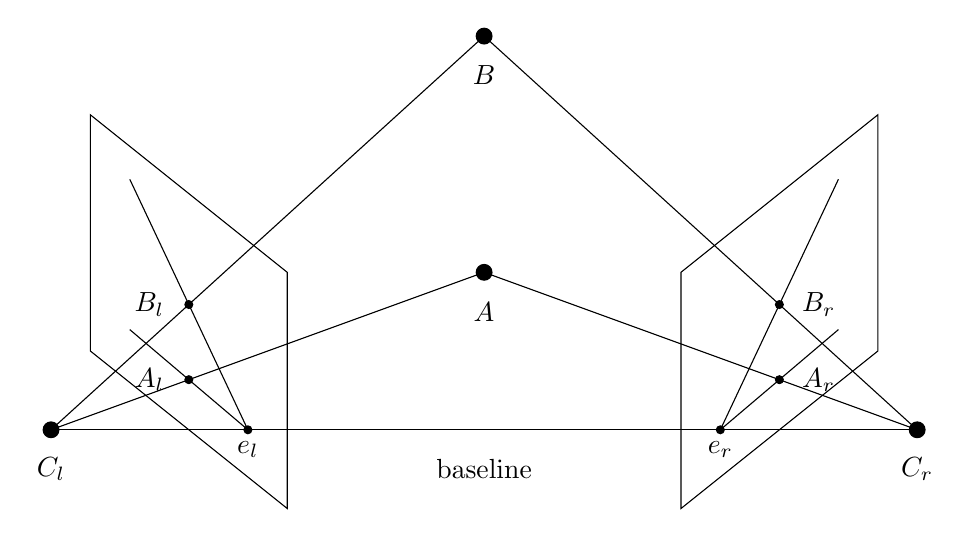
\begin{tikzpicture}[scale=0.5]
	% cameras
	\draw[fill] (-11,-1) circle [radius=0.2];
	\draw[fill] ( 11,-1) circle [radius=0.2];
	\draw (-11,-1) -- (11, -1);
	\node at (0, -2) { baseline };

	\node at (-11,-2) {$C_l$};
	\node at ( 11,-2) {$C_r$};

	% planes
	\draw (-10,1) -- (-10,7) -- (-5,3) -- (-5,-3) -- cycle;
	\draw ( 10,1) -- ( 10,7) -- ( 5,3) -- ( 5,-3) -- cycle;

	% 3d pts
	\draw[fill] ( 0,3) circle [radius=0.2];
	\draw[fill] ( 0,9) circle [radius=0.2];
	\node at (0,2) {$A$};
	\node at (0,8) {$B$};

	% origins via pts
	\draw (-11,-1) -- (0,3) -- (11,-1);
	\draw (-11,-1) -- (0,9) -- (11,-1);

	% epis
	\draw[fill] (-6,-1) circle [radius=0.1];
	\draw[fill] (6,-1) circle [radius=0.1];
	\node at (-6,-1.5) { $e_l$ };
	\node at (6,-1.5) { $e_r$ };

	% projections
	\draw[fill] (-7.5,0.2727) circle [radius=0.1];
	\draw[fill] (-7.5,2.1818) circle [radius=0.1];
	\node at (-8.5, 0.2727) {$A_l$};
	\node at (-8.5, 2.1818) {$B_l$};
	% lines from epis
	\draw (-6,-1) -- +(-2*1.5,2*1.2727);%(-7.5,0.2727);
	\draw (-6,-1) -- +(-2*1.5,2*3.1818);%(-7.5,2.1818);

	\draw[fill] (7.5,0.2727) circle [radius=0.1];
	\draw[fill] (7.5,2.1818) circle [radius=0.1];
	\node at (8.5, 0.2727) {$A_r$};
	\node at (8.5, 2.1818) {$B_r$};
	\draw (6,-1) -- +(2*1.5,2*1.2727);%(7.5,0.2727);
	\draw (6,-1) -- +(2*1.5,2*3.1818);%(7.5,2.1818);
\end{tikzpicture}
}{fig:epigeom}
{Epipolar geometry.
World points $A$, $B$ project to planes of different views imaged from $C_l$ and $C_r$ on the left ($A_l$ and $B_l$), and to the right ($A_r$, $B_r$).
When $A_l$ is known, its corresponding point $A_r$ (not initially known in practice) is found on the epipolar line joining $e_r$ and $A_r$ in the right image.
All epipolar lines in a view join in the same point ($e_l$ and $e_r$).}

Triangulation or reconstruction of the scene structure given by image pair(s) is usually done on the base of a known relationship between the cameras.
Such relationship, known as calibrating the cameras, can be automatically determined, given by X corresponding points that can be distinguished in each image and matched [?].
Commonly the points are particular \textit{features}, commonly very noticiable edges or corners, found with an algorithm such as SIFT [?], SURF [?] or Harris corner detector [?].

In stereo vision, the same scene of interest is seen by two or more cameras at the same time.
The cameras are rarely aligned perfectly such as in the setup described above, however.
Epipolar geometry encodes the relations between arbitrarily positioned cameras in a standard way so that coordinates of a 3D point seen in several images can be calculated with triangulation.

The locations and sensor planes of these cameras is related something

Projective stereo matching in most general case is underconstrained unless some real-world assumptions are fixed.



A point seen by camera A at 3d point P could be anywhere on the line between A's origin and P, because a certain line passing through the principal point always projects to a point.
This line is seen as a single point.
From another viewpoint in camera B, this line equals to some line on B's image plane.
The real point must be on that line.
The inverse applies for any point on B and a line on A.
The lines on the image planes are called epipolar lines.


Essential matrix defines how the camera poses differ by the something something points seen by both. $p_l$, $p_r$ 3d points; vectors from camera origins (camera coordinates!) to the same point (in camera coordinates):

\[ \label{eq:essential}
	p_r = R (p_l - t) \\
	p_r^T R T p_l = 0 \\
	p_r^T E p_l = 0
\]

where $T$ is the cross-product blahblah encoded in a matrix form below, essential matrix $E = R T$.

Le image. lecture11.pdf. O->p dot (O->O' cross O'->p') = 0

Cross product expressed in a skew-symmetric matrix form is
\begin{equation}
\vec a \times \vec b =
\begin{pmatrix}
	 0   & -a_z &  a_y\\
	 a_z &  0   & -a_x\\
	-a_y &  a_x & 0
\end{pmatrix}
\begin{pmatrix}
	b_x\\b_y\\b_z
\end{pmatrix}
= \vec c
\end{equation}

Fundamental matrix relates the corresponding points in stereo images; it has the same meaning as the essential matrix, but it works in the pixel coordinates of the cameras, which are obtained after the projective transform that takes the intrinsics into account.

Inverting the matrix $M_p$ in sensor-to-pixel coordinate transform

\[
\hat p_l = M_p p_l\\
\hat p_r = M_p p_r
\]

and using it on pixel coordinates, the world coords can be obtained, plugging in to the equation \ref{eq:essential}

\[
p_r^T E p_l = 0\\
(M_p^-1 \hat p_r)^T E (M_p^-1 \hat p_l) = 0\\
\hat p_r^T M_p^-T E M_p^-1 p_l = 0\\
\hat p_r^T F \hat p_l = 0
\]

the fundamental matrix

\[
F = M_p^-T E M_p^-1 = M_p^-T R T M_p^-1
\]

is obtained. It relates the pixels and epipolar lines, and as such it is useful in image processing where the images are described as pixels in a color array (image) and not colored physical coordinates.

Epipole can be interpreted as the location of another camera as seen by other camera.

\subsubsection{Point matching}

Previously, methods for reconstructing three-dimensional location for a point pair were introduced, assuming known positions for the same point in different images.
To reconstruct a whole scene from a full image, all pairwise points must be matched.

Matching can be done in sparse or dense mode; sparse matching finds a set of \textit{features} from each image, and tries to match them. Dense matching runs through each pixel of one image and tries to find the same from another one; from the coordinate differences between the two images, a disparity map is built. The disparities can be directly transformed to depth values.


\subsubsection{Correspondence and rectification}

In order to triangulate a real point from two or more photos, the location of the point in all images must be known.
Given a pixel in one image, what is the corresponding pixel in another image taken from the same scene?

Rectification is a process that simplifies this search problem by restricting the search to a single dimension.
By aligning the cameras such that their images are coplanar, the search only has to be performed on a line that is parallel to the line connecting the camera centers.
Usually, the calibration between the cameras is known at this point, and foobar.
After rectification, the corresponding lines are axis-aligned (horizontal or vertical) in both images.


\subsubsection{Multi-view stereo}

Multiple baseline stereo \cite{okutomi1993multiple}

\subsubsection{Structure from motion}

Structure from motion (SfM) refers usually to recovering the structure of a scene from the motion of a single camera.
For each view, the pose of the camera is determined and the scene structure is extended with the new information in the image.
(pollefeys)
Bundle adjustment is used to refine the camera parameters.

\subsubsection{Post-processing}

Uv mapping. Manual work. 3d noise removal; ignore points that have no close pair in other clouds.

Rendering: "as usual".

Post: remodel the mesh (face), see what it would look like. Refine parameters to get a similar output as in the photos (normal map etc.), backproject. Use colors and highpass them; assume uniform lightning and locally uniform texture color (bradley). (Simply a rendering technique, that level of detail in 3D structure might not be needed). Still, structured light and/or shading assumptions [shape from single image cues/shading trucco,verri p.225] done too.


\subsubsection{Reprojection errors}

The quality of the reconstruction is measured by reprojecting the 3D points back to the cameras and calculating the distance between the projected and original point.
Minimizing all of the points is very expensive but something something bundle adjustment.

Compare to algebraic, geometric etc.

A common way to handle feature errors is Random Sample Consensus (RANSAC). Random subsets of the sample space is iterated, and samples that do not fit well to a model that is constructed of a smaller set are ignored. The iteration that matches most samples is selected.

\subsection{Optical flow}

Long history; several mature commercial video editing products. The Matrix.

Uses: Frame time offset compensation by interpolation (morphing), needs features, direction vector estimation

